% Chapter 2

\chapter{Source localization with multi-scale dictionaries} % Main chapter title

\label{chapter:multiscale} % For referencing the chapter elsewhere, use \ref{Chapter1} 
\noindent\makebox[\linewidth]{\rule{0.75\paperwidth}{0.4pt}}
\noindent\makebox[\linewidth]{\rule{0.75\paperwidth}{0.4pt}}

\localtableofcontents % local toc

\noindent\makebox[\linewidth]{\rule{0.75\paperwidth}{0.4pt}}
\noindent\makebox[\linewidth]{\rule{0.75\paperwidth}{0.4pt}}
\newpage

%----------------------------------------------------------------------------------------
\section{Introduction}
In chapter~\ref{chapter:background}, we have seen all the background of the inverse problem in the MEG and EEG field. We justified the motivation for having sparse priors as regularization for the regression problem. Sparse priors were presented under different approaches. This chapter considers the variational problem in the Time-Frequency domain by fixing the penalization term as a sparse group LASSO as in Equation~\eqref{eq_sglasso}, with $\lambda_1$ a hyperparmeter over space, and $\lambda_2$, a second hyperparameter over time. Figure~\ref{fig:set_norms} justifies this choice. It shows how $\ell_{21}+\ell_1$ allows for modeling non-stationary sources which cannot be estimated with $\ell_2$ or $\ell_{21}$ due to the non-convexity promoting $\ell_2$-norm, while the $\ell_1$ estimate is completely scattered and unstructured.\\

\begin{figure}
\centering
	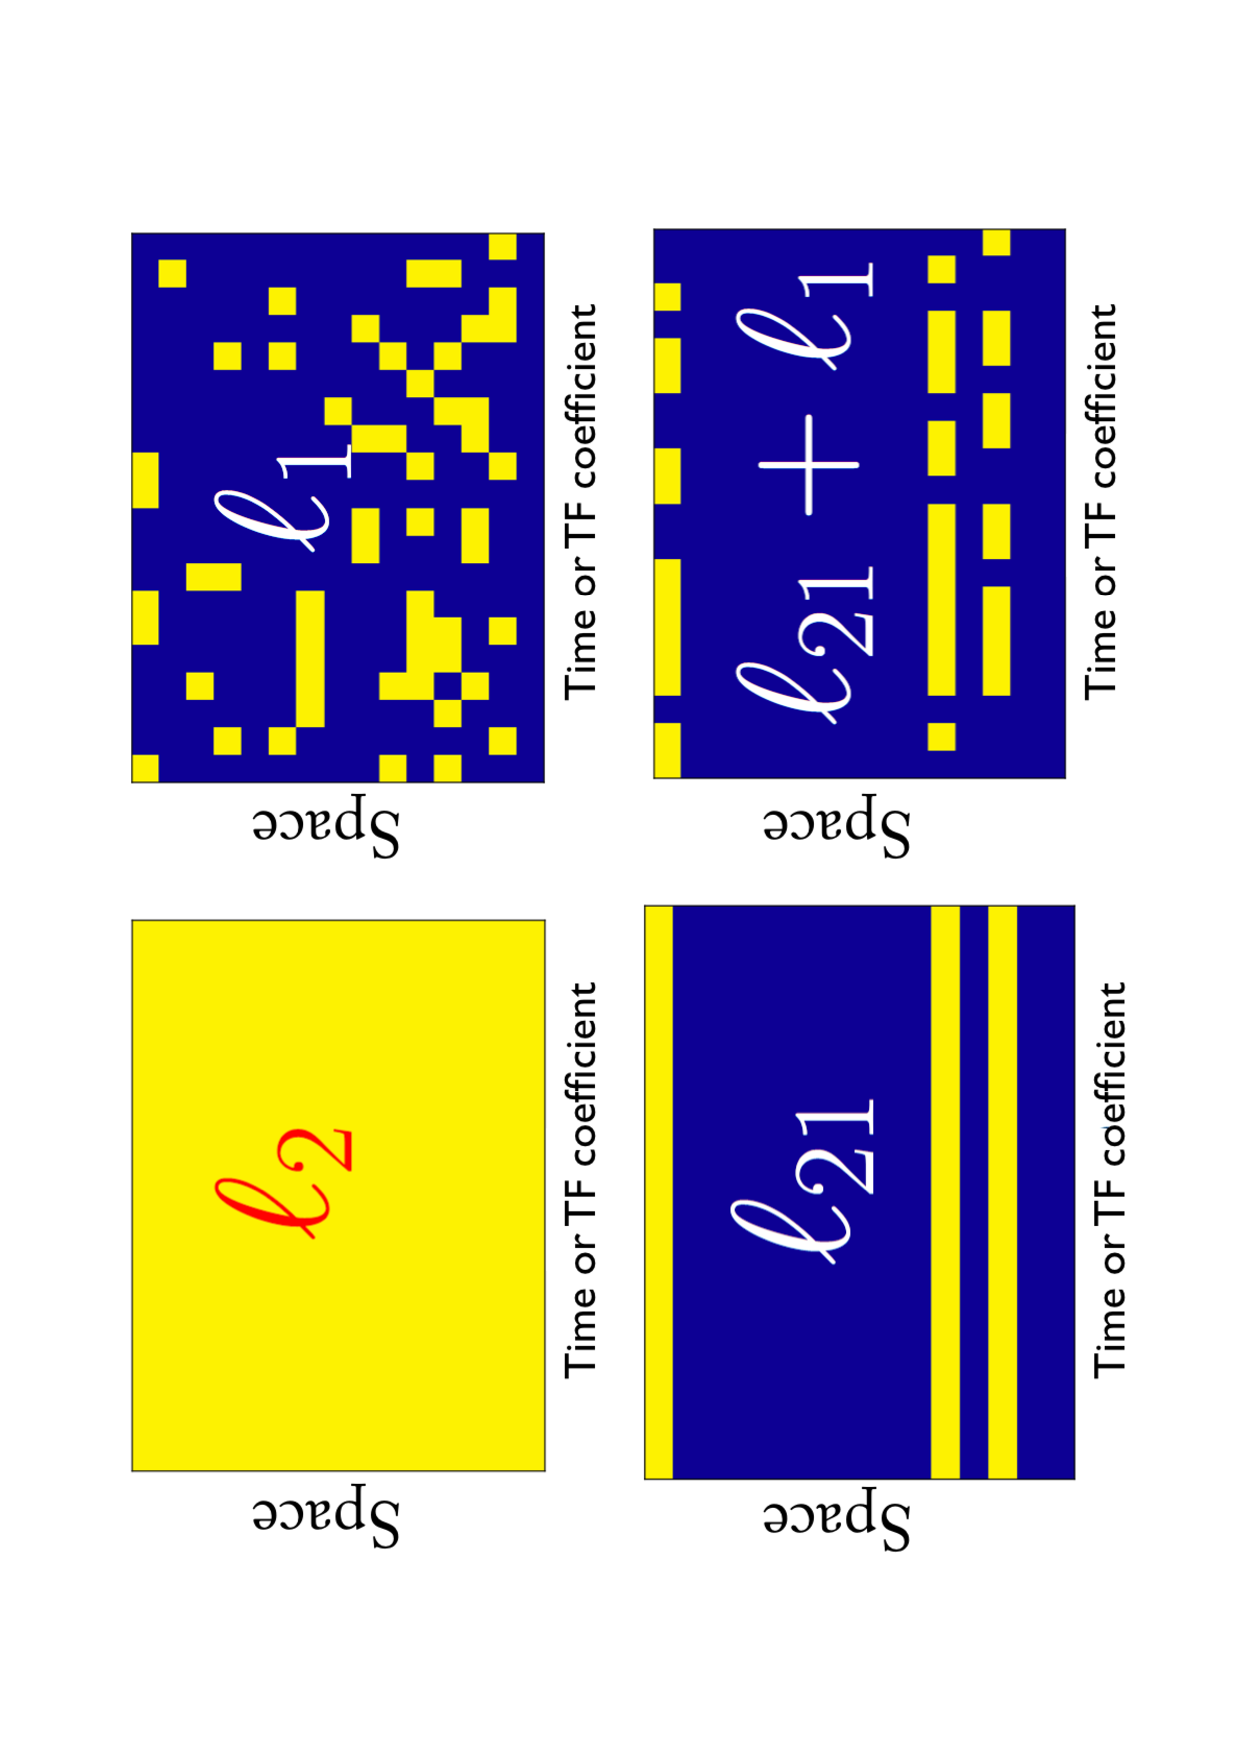
\includegraphics[angle=270,width=0.9\textwidth]{multidict/set_norms}
    \caption{Sparsity patterns promoted by the different regularizations: $\ell_2$ all non-zero, $\ell_1$ scattered and unstructured non-zero, $\ell_{21}$ block row structure, and $\ell_{21} + \ell_1$ (TF domain) block row structure with intra-row sparsity. Yellow color indicates non-zero coefficients.}
    \label{fig:set_norms}
\end{figure}

This chapter describes the source localization in the Time-Frequency (TF) domain. We have showed why localizing the source in the TF domain was a "true" spatio-temporal approach taking the time correlation into account.
The Time-Frequency Mixed Norm Estimate (TF-MxNE) \cite{Alex13}, Spatio-Temporal Unifying Tomography (STOUT) \cite{castano2015solving} and the iterative reweighted TF-MxNE (irTF-MxNE) \cite{daniel15} improve reconstruction of transient and non-stationary sources by promoting structured sparsity in the TF domain. Those methods compute a sparse group lasso on the TF coefficients. TF-MxNE and STOUT apply a composite convex penalty, the sum of an $\ell_{2, 1}$-mixed-norm and an $\ell_{1}$-norm penalty, on the Gabor transform of the source time courses. On the other hand, irTF-MxNE applies a composite \emph{non-convex} penalty, the sum of an $\ell_{2, 0.5}$-quasinorm and an $\ell_{0.5}$-quasinorm penalty on the TF coefficients.
The non-convex penalties have been shown to outperform convex approaches both in terms of source recovery and amplitude bias \cite{candes2008enhancing,daubechies2010iteratively} as explained in Chapter~\ref{chapter:background}. However, the choice of an optimal Gabor dictionary for decomposing the data remains difficult.\\

This issue of the choice of the dictionary is specially encountered when a mixture of signals is available in the data, \textit{e.g.}, short transient signal right after the onset of a stimuli, and slower brain waves afterward. A choice of a unique dictionary describing both signals in a sparse way is hard. We show in this chapter how to incorporate a multi-scale dictionary in the iterative reweighted optimization algorithm, \textit{i.e.} multiple dictionaries with different scales concatenated to fit short transients and slow waves at the same time, while keeping computational efficiency. The optimization problem is solved in the same way as irTF-MxNE \cite{daniel15}, \textit{i.e.}, each iteration is a weighted TF-MxNE, which we solve using block coordinate descent (BCD) and an active set strategy \cite{friedman2010regularization}. %We compare irTF-MxNE with and without a multi-scale dictionary on simulated and real MEG data. %As both solvers are able to recover the active set size,
We demonstrate the benefit of the multi-scale dictionary in terms of reconstructed source time courses and temporal unmixing of activations.

\section{Inverse problem in the Time-Frequency domain} \label{irtfmxne}

Using a dictionary of TF atoms, such as a tight Gabor frame, $\mathbf{\Phi} \in \mathbb{C}^{T \times C}$ ($T$ samples, $C$ atoms), the neuronal activation $\mathbf{X} \in \mathbb{R}^{SO \times T}$ ($S$ sources, $O$ orientation) can be modeled as a linear combination of atoms, $\mathbf{X}=\mathbf{Z\Phi}^{\mathcal{H}}$, where $\mathbf{Z} \in \CC^{SO \times C}$ is the TF coefficients matrix. A Gabor frame $\mathbf{\Phi}$ is tight (section~\ref{section:TF}) when the Euclidean norm of the input signal and the vector of TF coefficients are proportional ($\|\mathbf{Z}\|_2^2 = A_\mathbf{\Phi} \|\mathbf{X}\|_2^2$ where $A_\mathbf{\Phi}>0$). When $A_\mathbf{\Phi}=1$ the frame is said to be normalized. We will use tight frames in the following.

The MEG/EEG measurements $\mathbf{M} \in \mathbb{R}^{N \times T}$ ($N$ sensors) follows the forward model:
\begin{equation} \label{eq:reg_prob_tf}
    \mathbf{M} = \mathbf{GX} + \mathbf{E} = \mathbf{GZ \Phi}^{\mathcal{H}} + \mathbf{E}
\end{equation}

where $\mathbf{G} \in \mathbb{R}^{N \times SO}$ stands for the forward operator. $\mathbf{E} \in \mathbb{R}^{N \times T}$ is the measurement noise, which can be assumed to be additive white noise: $\mathbf{E}[:, j] \sim \mathcal{N}(0, \mathbf{I})$ for all $j$ after spatial whitening \cite{denis}. Estimating the coefficients $\mathbf{Z}$ given the measurement $\mathbf{M}$ is an ill-posed problem and constraints have to be imposed on $\mathbf{Z}$ to obtain a unique source estimate, as described for $\mathbf{X}$ in the last chapter. For analyzing evoked responses, we assume that the neuronal activation is spatially sparse and temporally smooth. This corresponds to a row sparsity~\cite{Alex13}, which we promote by applying a composite non-convex regularization $\mathcal{P}(\mathbf{Z})$ (See Figure~\ref{fig:set_norms}). The associated regularized regression problem is:
\begin{equation} \label{eq:penalized_reg_tf}
    \mathbf{Z}^\star = \argmin_{\mathbf{Z}} \frac{1}{2}\|\mathbf{M - GZ\Phi^\mathcal{H}}\|^2_{Fro} + \mathcal{P}(\mathbf{Z})
\end{equation}
with
\begin{equation}
%\begin{split}
%	\mathcal{P}(\mathbf{Z}) & = \lambda_{space}\mathcal{P}_{1}(\mathbf{Z}) + \lambda_{time}\mathcal{P}_{2}(\mathbf{Z}) \\
%& = \lambda_{space}\|\mathbf{Z}\|_{2,0.5} + \lambda_{time}\|\mathbf{Z}\|_{0.5} \\
%\end{split}
	\mathcal{P}(\mathbf{Z}) = \lambda_{space}\|\mathbf{Z}\|_{2,0.5} + \lambda_{time}\|\mathbf{Z}\|_{0.5}
\end{equation}
where $\lambda_{space} > 0$, $\lambda_{time}>0$. A large regularization parameter $\lambda_{space}$ will lead to a spatially very sparse solution or even an empty solution, while a large $\lambda_{time}$ will promote sources with smooth time series and might loose sharp aspect of the neural activity.

\section{Fast iterative reweighted TF-MxNE with tight frames}
Given a dictionary $\mathbf{\Phi}$, the optimization problem in Equation~\eqref{eq:penalized_reg_tf} can be solved by iteratively minimizing convex surrogate problems~\cite{daniel15}. The regularization term at each iteration $k$ is a weighted convex mixed norm that can be written as:
\begin{equation} \label{eq:weights_optim}
%   \mathcal{P}(\mathbf{Z}) = \lambda_{space}\sum_{s}\sqrt{\|\mathbf{Z}[s,:]\|_2} + \lambda_{time}\sum_{s,c}\sqrt{|\mathbf{Z}[s,c]|}
    \mathcal{P}(\mathbf{Z}) = \lambda_{space}\|\mathbf{Z}\|_{\mathbf{W}_1^{(k)};2,1} + \lambda_{time}\|\mathbf{Z}\|_{\mathbf{W}_2^{(k)};1}
\end{equation}
with $\forall s,c$,
\begin{equation*}
\begin{aligned}
    \mathbf{W}_1^{(k)}[s,c] &= \left(2\sqrt{\|\hat{\mathbf{Z}}^{(k-1)}[s,:]\|_2 + \epsilon^{(k-1)}}\right)^{-2} \\
    \mathbf{W}_2^{(k)}[s,c] &= \left(2\sqrt{|\hat{\mathbf{Z}}^{(k-1)}[s,c]| + \epsilon^{(k-1)}}\right)^{-1}
\end{aligned} \enspace ,
\end{equation*}
%
where $\mathbf{W}_1$ and $\mathbf{W}_2$ are the weights applied to the TF coefficients, and $\mathbf{\hat{Z}}^{(k-1)}$ are the estimated coefficients at iteration $(k-1)$. $\epsilon^{(k-1)} \in \mathbb{R}^+$ is used to prevent infinite weights. To have an intuition about the update rule for the weights, one can prove that updating the weights with $w_i$=$|x_i|^{p-2}$ leads to a solution of the $\ell_p$-norm penalized problem.\\
%Here, $\epsilon$ is set to $0$ and infinite weights are handled as in \cite{daniel15}.

For solving Equation~\eqref{eq:penalized_reg_tf}, we use BCD~\cite{tseng2010approximation}. The algorithm boils down to sequentially computing a gradient step and the proximity operator of the $\ell_{2,1}+\ell_1$ norm for each block $s$ of coefficients (See Section~\ref{section:BCD}). Here a block maps to a location in the brain. One update of a block of coefficients is given by first a gradient step:
\begin{align} \label{eq:block_update}
    \mathbf{R} &= \mathbf{M} - \mathbf{G}\hat{\mathbf{X}} \\
    \bar{\mathbf{X}}[s,:] &= \hat{\mathbf{X}}[s,:] + \mathbf{\mu}[s]\mathbf{G}[:,s]^\top\mathbf{R} \\
    \bar{\mathbf{Z}}[s,:] &= \bar{\mathbf{X}}[s,:]\mathbf{\Phi}
    % \mathbf{R} &= \mathbf{M} - \mathbf{G}\hat{\mathbf{Z}}\mathbf{\Phi}^{\mathcal{H}} \\
    % \bar{\mathbf{Z}}[s,:] &= \hat{\mathbf{Z}}[s,:] + \mathbf{\mu}[s]\mathbf{G}[:,s]^\mathbf{T}\mathbf{R}\mathbf{\Phi} \\
\end{align}
followed by the computation of the proximity operator of the weighted $\ell_{2,1}+\ell_1$ described in Chapter~\ref{chapter:background}-Equation~\ref{prox_mixed}:
\begin{equation} \label{prox_l1}
\begin{aligned}
    \tilde{\mathbf{Z}}[s,c] &= \bar{\mathbf{Z}}[s,c]\left(1 - \frac{\mathbf{\mu}[s]\lambda_{time}\mathbf{W}_2^{(k)}[s,c]}{|\bar{\mathbf{Z}}[s,c]|} \right)_+
\end{aligned}
\end{equation}
\begin{equation} \label{prox_l21}
\begin{aligned}
    \hat{\mathbf{Z}}[s,c] &= \tilde{\mathbf{Z}}[s,c]\left(1 - \frac{\mathbf{\mu}[s]\lambda_{space}\sqrt{\mathbf{W}_1^{(k)}[s,c]}}{\|\tilde{\mathbf{Z}}[s,:]\|_2}\right)_+
\end{aligned}
\end{equation}
When $\mathbf{\Phi}$ is a tight frame, $\mathbf{\mu}[s]$ is the step length for each BCD subproblem and it is given by $\mathbf{\mu}[s]=\sqrt{\mathbf{A}_{\mathbf{\Phi}}}(\|\mathbf{G}[:,s]^T\mathbf{G}[:,s]\|)^{-1}$. This step length, \textit{i.e.} the inverse of the Lipschitz constant restricted to the source $s$ is typically larger than the step length applicable in iterative proximal gradient methods, which is upper bounded by $\|\mathbf{G}^T\mathbf{G}\|^{-1}$. This implies a bigger step to speed up the convergence.
Finally:
\begin{equation}
    \hat{\mathbf{X}}[s,:] = \hat{\mathbf{Z}}[s,:]\mathbf{\Phi}^\mathcal{H}
\end{equation}

Equation~\eqref{prox_l1} and \eqref{prox_l21} are respectively solutions of the proximity operator for the weighted $\ell_1$-norm and for the weighted $\ell_{2,1}$-norm. As the $\ell_1$ proximity operator shrinks coefficients towards zero, if a block of coefficients were set to zero by the $\ell_{2,1}$ proximity operator, it would also be set to zero after the application of the $\ell_1$ proximity operator. As a consequence, it is possible to know just by applying the $\ell_{2,1}$ proximity operator to $\bar{\mathbf{X}}[s,:]$ if the set of coefficients $\tilde{\mathbf{Z}}[s,:]$ will be set to zero. Note that this is just a sufficient condition and we may have to compute all steps to know if the block is set to zero. This is summarized in the following lemma.

\begin{lemma}
    Let $\mathbf{\Phi}$ be a frame with constant $A_{\mathbf{\Phi}}$, if $\|\bar{\mathbf{X}}[s,:]\|_2$ $\leq \mathbf{\mu}[s]\lambda_{space}\sqrt{\mathbf{W}_1^{(k)}[s,c]} / \sqrt{A_{\mathbf{\Phi}}}$ then $\hat{\mathbf{Z}}[s,c] = 0$, $\forall c$.
\end{lemma}

Computing the TF decomposition at each iteration can be costly. The consequence of the lemma is that for a lot of source locations one can avoid computing their TF decomposition during the optimization just by computing the $\ell_{2}$-norm of the time courses after the gradient step.
To speed up the computation even more, we combine the BCD scheme~\ref{section:BCD} with an active set strategy~\ref{section:active_set}~\cite{friedman2010regularization}, which primarily updates sources that are likely to be active, while keeping the remaining sources inactive.

\subsection*{Orientation constraints}
Let $\mathbf{Z}_s\in\CC^{3\times C}$ be the block of the $\mathbf{Z}\in\CC^{3S\times C}$	corresponding to the $s^{th}$ source and $\mathbf{Z}[1,:]$ being the activity of the dipole oriented normal to the cortical surface, and $\mathbf{Z}[2,:]$ and $\mathbf{Z}[2,:]$ the two other orientation tangent to the surface. We modify the $\ell_1$-norm and the $\ell_{2,1}$-norm for the free orientation constraints as follow:
\begin{align*}
\|\mathbf{Z}\|_1 &= \sum_{s,c}\sqrt{|\mathbf{Z}_s[1,c]|^2 + \frac{1}{\kappa^2}|\mathbf{Z}_s[2,c]|^2 + \frac{1}{\kappa^2}\mathbf{Z}_s[3,c]|^2} \\
\|\mathbf{Z}\|_{2,1} &= \sum_s\sqrt{\sum_c |\mathbf{Z}_s[1,c]|^2 + \frac{1}{\kappa^2}|\mathbf{Z}_s[2,c]|^2 + \frac{1}{\kappa^2}\mathbf{Z}_s[3,c]|^2}
\end{align*}
where $s$ indexes the source location and $c$ the TF coefficient. When $\kappa=1$, no orientation contraint is applied and the modified penalties amount to grouping the orientation in a common $\ell_2$-norm.

\section{Inverse problem with multi-scale tight Gabor frames}
A tight Gabor frame is computed by setting two parameters: the length of the window (window size), and an overlap parameter (time shift). The window size defines the time/frequency resolution, if its length is short, it would be more focus on time than frequency, and vice versa, if it is long, it will be more focus on frequency than in time. The time resolution also depends on the time shift parameter. The time shift parameter defines the time step from one window to another (section~\ref{section:TF}). This affects the redundancy of the dictionary. A dense sampling of the TF space, however, increase the complexity on both time and memory.\\

Each source waveform is a sparse linear combination of atoms from this dictionary. Fixing those parameters is then critical for having an optimal dictionary. %This makes the choice of the parameters important when they are fixed and not learned.
Learning the dictionary might be a solution to avoid fixing the parameters, or the need to have an overcomplete dictionary covering a broad range of scales. However, learning both $\mathbf{Z}$ and $\mathbf{\Phi}$ simultaneously is a non-convex optimization problem, for which one needs to alternate between a convex optimization for the two variables~\cite{montoya2014regularized}. \\

%Setting the number of atoms to be learned and the stopping criterion is also challenging.

Let us define a multi-scale TF dictionary, where we concatenate $Q$ tight Gabor frames $\mathbf{\Phi}_q$, $ 1 \leq q \leq Q$, with different resolutions. One can realize that this union of tight frames $\mathbf{\Phi} = [\mathbf{\Phi}_1, \dots, \mathbf{\Phi}_Q]$ is also a tight frame with $A_\mathbf{\Phi} = \sum_q A_{\mathbf{\Phi}_q}$. The strategy presented in the previous section~\ref{irtfmxne} is therefore still relevant for a multi-scale dictionary, where the activation $\mathbf{Z}$ is a concatenation of $\mathbf{Z}_1, \mathbf{Z}_2, ..., \mathbf{Z}_Q$. Algorithm~\ref{alg:multiscale_tfmxne_activeset} describes how to solve the inverse problem in the TF domain with a multi-scale dictionary.

{\fontsize{4}{4}\selectfont
%above is to make smaller fonts in algorithm
\begin{algorithm}[t]
\SetKwInOut{Input}{input}
\SetKwInOut{Init}{init}
\SetKwInOut{Parameter}{param}
\caption{\textsc{multi-scale TF-MxNE with active set strategy}}
\Input{$\bfM, \bfG, \mathbf{\Phi}=[\mathbf{\Phi}_1, \dots, \mathbf{\Phi}_Q], \lambda_{space} > 0, \lambda_{time}$, and $\epsilon>0$}
% \Parameter{ To add }
\Init{$\mathbf{Z}\in\RR^{SO\times C}$, $\Gamma=\{\}$, $\eta=f_p(\mathbf{Z})-f_d(\mathbf{Y})$, $\mathbf{\mu}$ with $\mathbf{\mu}[s]=\mathcal{L}^{-1}_s=\|\mathbf{G}_s^\top\mathbf{G}_s\|^{-1}$}
\While{
		$\eta \geq \epsilon$
	  }
	  {
	  	$\Gamma^\star \subseteq {s \hspace{3pt} | \hspace{3pt} \|Prox_{\lambda_{time}\|.\|_1}(\mathbf{G}_s^\top(\mathbf{M}-\mathbf{GZ\Phi}\mathcal{H})\Phi)\|_{Fro} > \lambda_{space} }$
	  	
	  	$\Gamma = \Gamma \cup \Gamma^\star$
	  	
	  	$\mathbf{Z}^{\star\Gamma}\leftarrow$ Solve Algorithm~\ref{alg:multiscale_tfmxne_bcd} with $\mathbf{\mu}$, and $\Gamma$
	  	
	  	$\mathbf{Z}=\mathbf{Z}^{\star\Gamma}$ for $i\in\Gamma$, else 0

	  	$\eta=f_p(\mathbf{Z})-f_d(\mathbf{Y})$
	  }
\label{alg:multiscale_tfmxne_activeset}
\end{algorithm}
}

{\fontsize{4}{4}\selectfont
%above is to make smaller fonts in algorithm
\begin{algorithm}[t]
\SetKwInOut{Input}{input}
\SetKwInOut{Init}{init}
\SetKwInOut{Parameter}{param}
\caption{\textsc{multi-scale TF-MxNE with BCD}}
\Input{$\bfM, \bfG, \mathbf{\Phi}, \mathbf{\mu}, \lambda_{space} > 0, \lambda_{time} > 0, \epsilon > 0$, and $\Gamma^\star$ }
% \Parameter{ To add }
\Init{$\eta=f_p(\mathbf{X})-f_d(\mathbf{Y})$}
\While{
		$\eta \geq \epsilon$
	  }
	  {
	  	\For{
	  			$s\in\Gamma^\star$
	  		}
	  		{
	  			$\mathbf{Z}_s = Prox_{\mathbf{\mu}[s](\lambda_{space}\|.\|_{2,1}+\lambda_{time}\|.\|_1)}(\mathbf{Z}_s+\mathbf{\mu}[s]\mathbf{G}^\top_s(\mathbf{M}-\mathbf{GZ\Phi}^\mathcal{H})\mathbf{\Phi})$
	  		}
	  	$\eta = f_p(\mathbf{X})-f_d(\mathbf{Y})$
	  }
\label{alg:multiscale_tfmxne_bcd}
\end{algorithm}
}


\section{Experiments with different dictionaries}
%----------------------------------------------------------------------------------------
We first evaluate the accuracy of irTF-MxNE with and without multi-scale on realistic simulations. We then apply our new solver on MEG somatosensory data.

\subsection{Simulation}
We generated a realistic simulation dataset based on a fixed-orientation source model with 7549 cortical locations and 102 magnetometers. Two of these locations were selected to be active in the primary and secondary somatosensory cortex (S1 and S2). The corresponding time courses are shown in Fig. \ref{fig:simulation}-a in blue (S1) and green (S2). We have both a transient source around 40 ms and slow waves afterwards around 70, 100 and 150 ms. The irTF-MxNE solver improves the source recovery \cite{daniel15}. Therefore, we do not compare the solvers presented here over the active set size or an $F_1$ measure, %(based on the Recall and Precision)
as both solvers are already able to recover all the sources. % due to the \textit{non-convex} optimization.
We evaluate our approach by computing  %$RMSE=\|X_{sim}-X_{est}\|_{Fro}$ and
the explained variance between simulated source courses and the source estimation from each solver as follows:
\begin{equation}
	\theta = 1 - \frac{\|GX_{sim}-GX_{est}\|^2_{Fro}}{\|GX_{sim}\|^2_{Fro}} \enspace
\end{equation}

Fig.~\ref{fig:simulation}-b shows the explained variance for the irTF-MxNE with different dictionaries over a logarithmic grid of $\lambda_{space}$. The first Gabor dictionary is constructed with 64 samples (64 ms) window and 4 samples time shift (green), the second Gabor dictionary is constructed with 16 samples window and 2 samples time shift (red) and the third one is the combination of the two dictionaries (blue). We observe that the irTF-MxNE solver using the combination of two dictionaries outperforms the solver with each dictionary separately in terms of explained variance measure over all parameters range. Higher values of $\log(\lambda_{space})>1.2$ impose high penalization on the active set size, resulting in a too sparse source estimate, where the solution does not explain the measurement anymore. The results show on simulation a source reconstruction improvement, where it leads to a larger explained variance.

\begin{figure}
\centering
	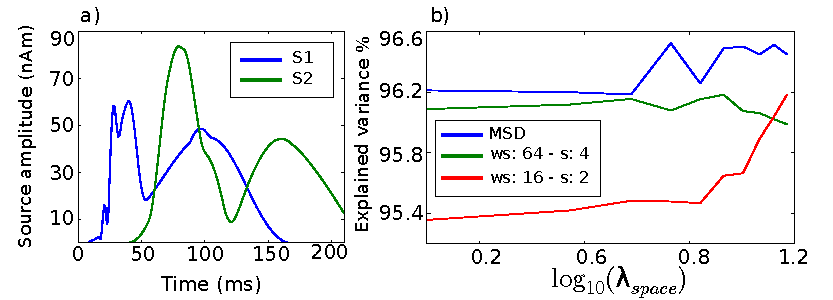
\includegraphics[width=0.85\textwidth]{multidict/fig_sim}
    \caption{(a) Simulated source time courses in S1 (blue) and S2 (green). (b) The explained variance for irTF-MxNE using two different dictionaries: long window size (ws) 64 with time shift (s) 4 (green), and small ws 16 with s 2 (red). The combination of the two dictionaries is shown in blue. This shows how the multi-scale dictionary (MSD) improves the explained variance.}
    \label{fig:simulation}
\end{figure}

\subsection{Experimental results with MEG somatosensory data}
To demonstrate the advantage of irTF-MxNE with a multi-scale dictionary over the basic irTF-MxNE, we tested different parameters for different solvers on a MEG dataset: somatosensory study of the MIND dataset (for details \cite{weisend2007paving}). The evoked is shown in Figure~\ref{fig:evoked_mind}. One can already notice this mixture of brain waves in the evoked. Sharper waves right after the onset in the evoked are due to a nice alignment of the trials which their information is not lost after averaging. This is mainly known as a response of the primary somatosensory area (S1) which answers quickly after a painless electrical stimulation of the median nerve. It is clearly seen from the evoked also this longer wave which comes later around 70ms. This is what makes this data a challenging dataset and a very good one for testing the multi-scale solver.

\begin{figure}
\centering
	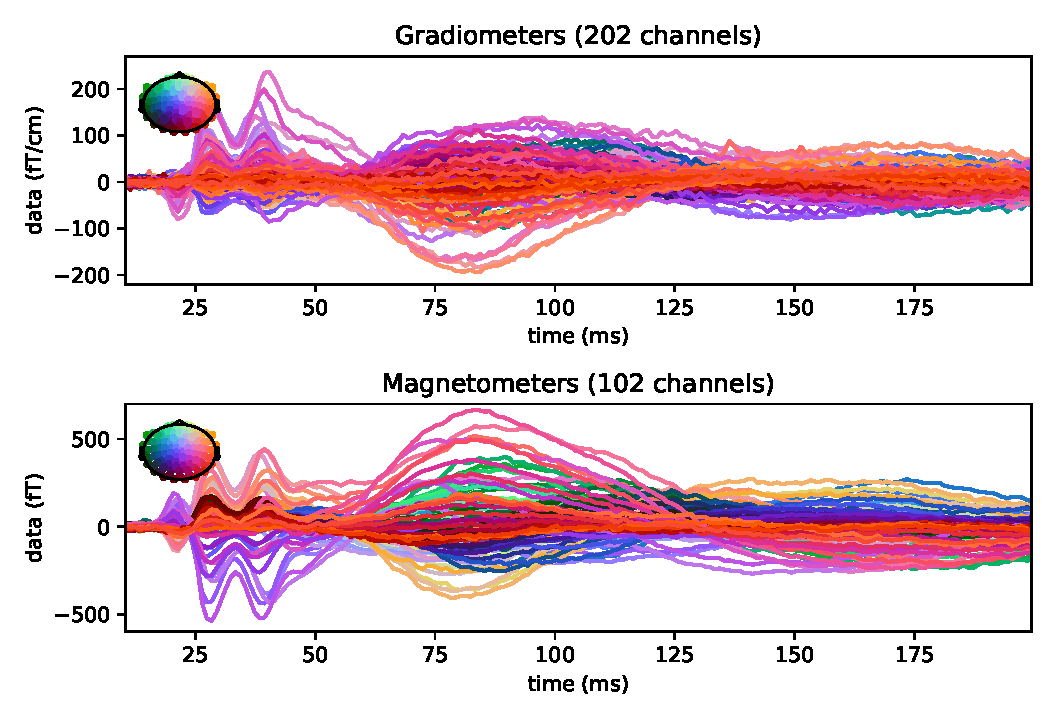
\includegraphics[width=0.9\textwidth]{multidict/evoked_mind_MEG}
    \caption{Somatosensory evoked response after preprocessing and averaging (gradiometers and magnetometers data).}
    \label{fig:evoked_mind}
\end{figure}

Source estimation was first performed using several solvers: irTF-MxNE, irMxNE~\cite{strohmeier2014iterative} and dSPM~\cite{dale2000dynamic}. Regarding irTF-MxNE, two dictionaries were tested (both STFT dictionaries). A dictionary with a 64 samples window and a 4 samples time shift, which leads to smooth source courses; and a dictionary with a 16 samples window and a 2 samples time shift, which helps capture short transient sources. After inspection of the residual in the Figure~\ref{fig:residual_mind}, results showed that at least four sources are necessary to capture all evoked components. 

We have therefore fixed the parameters of the irTF-MxNE solvers so we obtained only four sources while explaining as much variance as possible. After that, we experimented with a set of different parameters and we show two of them $\lambda_{time}=1.5$ and $\lambda_{time}=2.5$ to demonstrate their impact on the smoothness of the different time sources obtained.
The parameters were chosen in such a way to reduce the residual \textit{i.e.} to maximize the explained data by having at least four sources. 
Figure~\ref{fig:MEG_dics} (a-b) demonstrates the four time courses obtained with irTF-MxNE using the short window dictionary for the selected values of $\lambda_{time}$.

\begin{figure}
\centering
	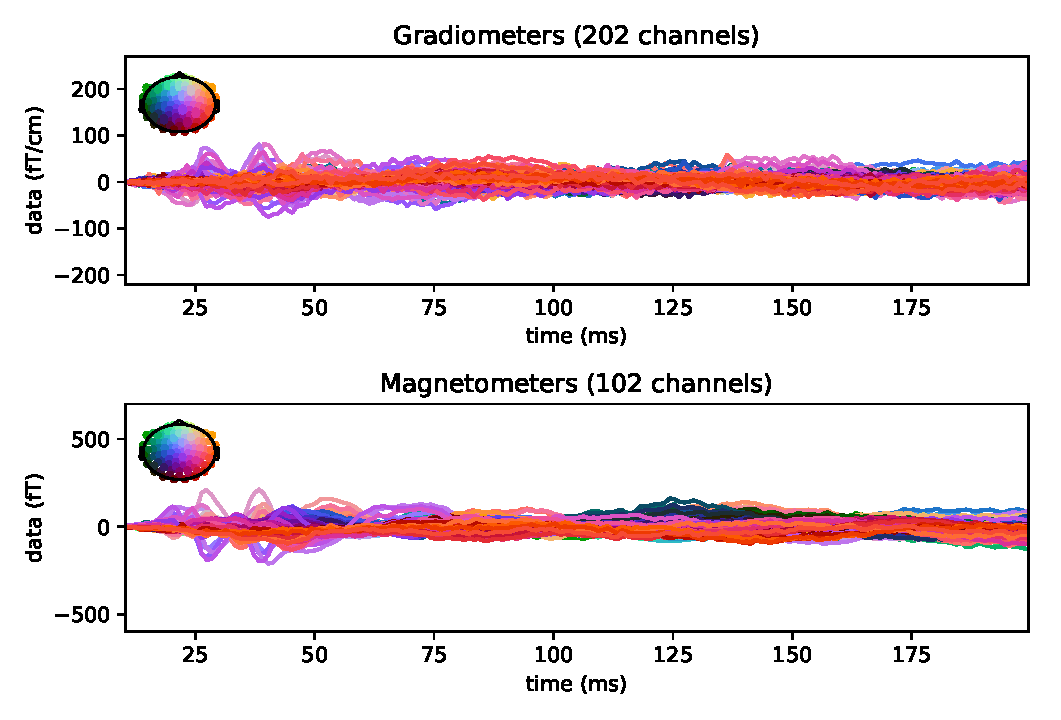
\includegraphics[width=0.9\textwidth]{multidict/residual_mind_MEG}
    \caption{Residual of the somatosensory data after applying the multi-scale irTF-MxNE.}
    \label{fig:residual_mind}
\end{figure}

We show that for high values of $\lambda_{time}$ (b), the solver is not able to capture the short transient component around 30 ms. While for a small value (a), the unmixing is not reliable since the light blue and the green source estimates catch the activity from the red source. Additionally, the time courses are not smooth. On the other hand, Figure~\ref{fig:MEG_dics} (c-d) demonstrate the four time courses obtained with irTF-MxNE using the long window dictionary for the selected $\lambda_{time}$. The figure confirms that both parameters are not able to capture the transient effect after the stimulus, although the time courses are smooth. These four sub-figures reveal that one need a short window to capture the transient effect of the brain signal (See Figure~\ref{fig:residual_long_dic}), while it needs to have a long window to capture the long waves and to have smooth source estimates. This result demonstrates how a combination of the two dictionaries is critical to acquire source estimates with high precision, but the hyperparameters needs to be tuned as well as shown in this Figure~\ref{fig:MEG_dics} that their values change drastically the results.

\begin{figure}
\centering
	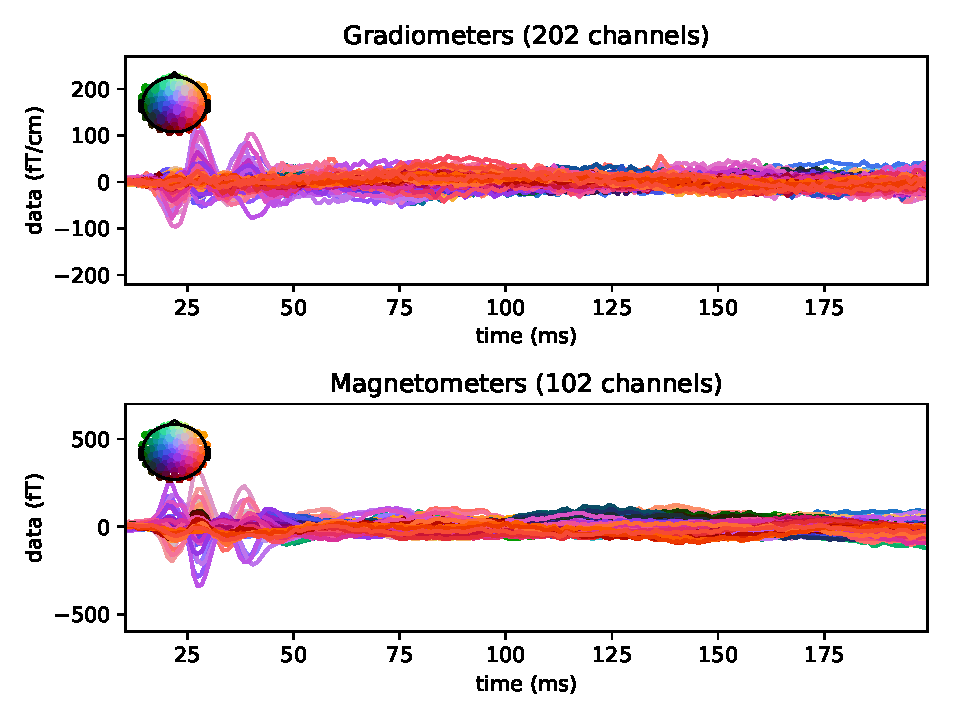
\includegraphics[width=0.9\textwidth]{multidict/residual_mind_MEG_long_dictionary}
    \caption{Residual of the somatosensory data after applying irTF-MxNE with a long window dictionary (window size = 64, time shift = 4). The transient part of the brain signal is left in the residual as it cannot be modeled by the long dictionary.}
    \label{fig:residual_long_dic}
\end{figure}

Moreover, Figure~\ref{fig:MEG_dics} (e) displays the amplitudes obtained with MxNE for five sources, as for MxNE, one is not able to obtain the four relevant sources unmixed (See for more demonstrative figures~\cite{gramfort2012mixed}). We notice that the light blue source in Figure~\ref{fig:MEG_dics} (a) to (d) appears as two separate sources in (e): light blue and purple. If we increase the $\lambda$ parameter, we increase the amplitude bias due to the $l_1$ norm of the solver. If we set it too high ($\lambda=50$) we obtain four sources, but the blue source which is relevant to the study would be removed and the duplicated purple source is kept. The last panel Figure~\ref{fig:MEG_dics} (f) displays the source estimates for dSPM values corresponding to the four locations of the sources obtained with the irTF-MxNE. These sub-figures show that none of MxNE or dSPM solvers are able to obtain smooth sources without any leakage between the time courses.

\begin{figure}
\centering
	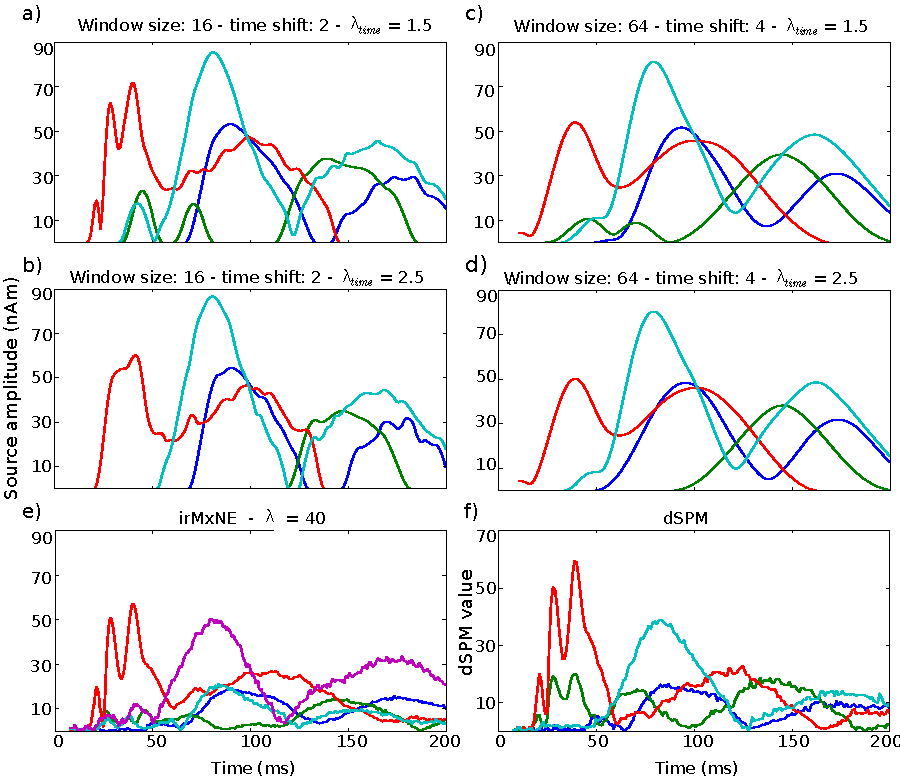
\includegraphics[width=0.95\textwidth]{multidict/fig_dics}
    \caption{Source reconstruction using somatosensory data with different solvers. (a) - (b) irTF-MxNE on a small window dictionary with $\lambda_{time}=1.5$ and $\lambda_{time}=2.5$ respectively. (c) - (d) irTF-MxNE on a long window dictionary with $\lambda_{time}=1.5$ and $\lambda_{time}=2.5$ respectively. From (a) to (d) $\lambda_{space}=28.5$ (e) MxNE for $\lambda=40$ and (f) dSPM activation for the four activated sources.}
    \label{fig:MEG_dics}
\end{figure}

Source estimation was then achieved using irTF-MxNE with the combination of the two dictionaries.
Figure~\ref{fig:MEG} shows source reconstruction using the multi-scale irTF-MxNE for the regularization parameters $\lambda_{space}=28.5$ and $\lambda_{time}=1.5$. Each source's location is marked by a sphere in Figure~\ref{fig:MEG} left, and its amplitude over time is color-coded in the right panel. The results show a suitable succession of the sources. The transient source (red) is the only source explaining the event related field until 48 ms. This red source corresponds to the contralateral primary somatosensory cortex (cS1) located in the postcentral gyrus of the parietal lobe (right hemisphere (rh)). The red sphere on the lateral view coincides with the smeared dSPM activation around 40 ms. The second source (light blue) corresponds to the secondary somatosensory cortex (cS2), and also occurs with dSPM activation around 80 ms. About 100 ms after stimulus, additional cortical sources are activated, such as ipsilateral secondary somatosensory cortex (iS2) (blue-lh), and contralateral medial wall (green-rh). 

\begin{figure}
\centering
	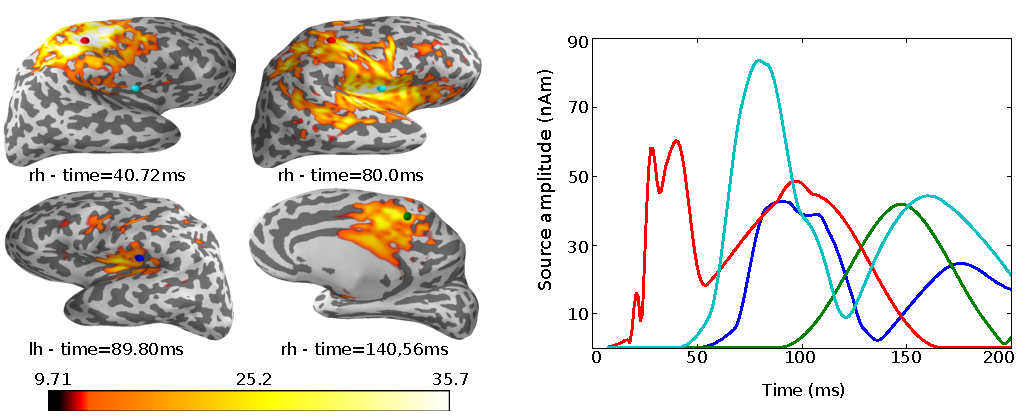
\includegraphics[width=0.95\textwidth]{multidict/fig_MEG}
    \caption{Source reconstruction using somatosensory data with a multi-scale irTF-MxNE. The solver estimates four sources for $\lambda_{space}=28.5$ and $\lambda_{time}=1.3$. The source locations marked with spheres in right (rh) and left (lh) hemisphere, and their corresponding activation are color-coded.}
	\label{fig:MEG}
\end{figure}

The multi-scale version of the MEG/EEG inverse problem in the TF domain does not only allow the capture of mixture of brain signals. An interesting point is the non-stationary aspect of the sources, which can be activated only for a short time window in a longer one. This multi-scale solver is then allowing us to analyze and reconstruct signals with variable characteristics over time. So far, all the results presented have been using a Gabor transform by fixing its window length and the time shift. The Gabor transform is a special case of STFT (the discrete case), and the question is what if this dictionary is not the best choice of where to decompose the data. The choice of the STFT was driven mostly by its flexibility of the choice of the dictionary being redundant or overcomplete. Moreover, its efficient implementation using fast FFT makes the STFT/iSTFT computation possible even with very redundant dictionaries.\\

\begin{figure*}
        \centering
        \begin{subfigure}[b]{0.48\textwidth}
            \centering
            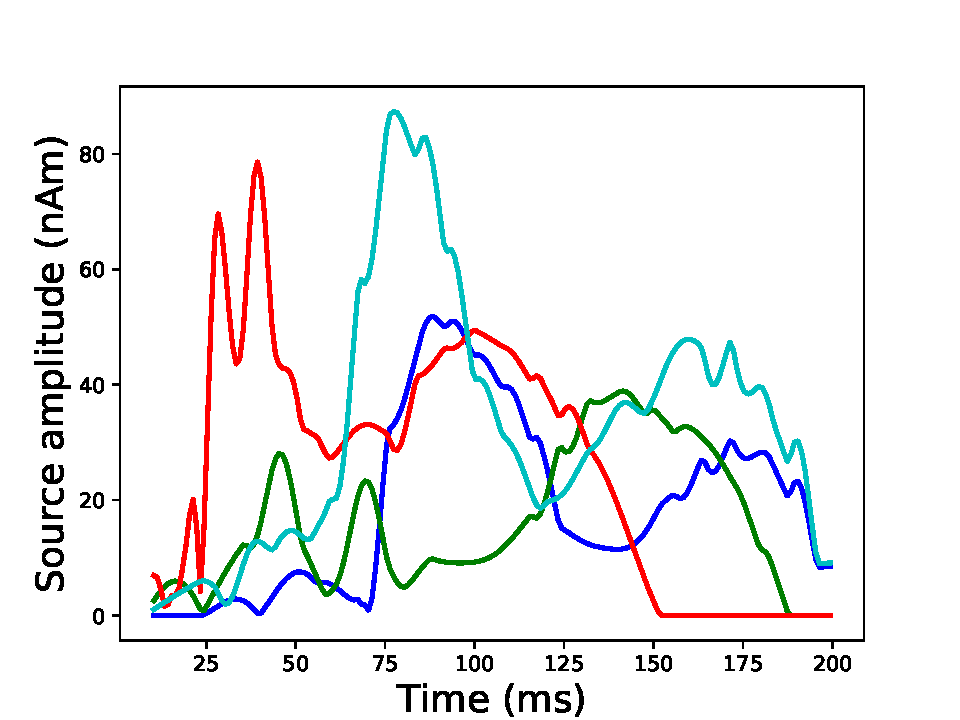
\includegraphics[width=\textwidth]{multidict/mdct_ws_64_16_tshift_32_8}
            \caption{MDCT: window size = 64-16,\\
            		    time shift = 32-8}
            \label{fig:mdct_short}
        \end{subfigure}
        \hfill
        \begin{subfigure}[b]{0.48\textwidth}  
            \centering 
            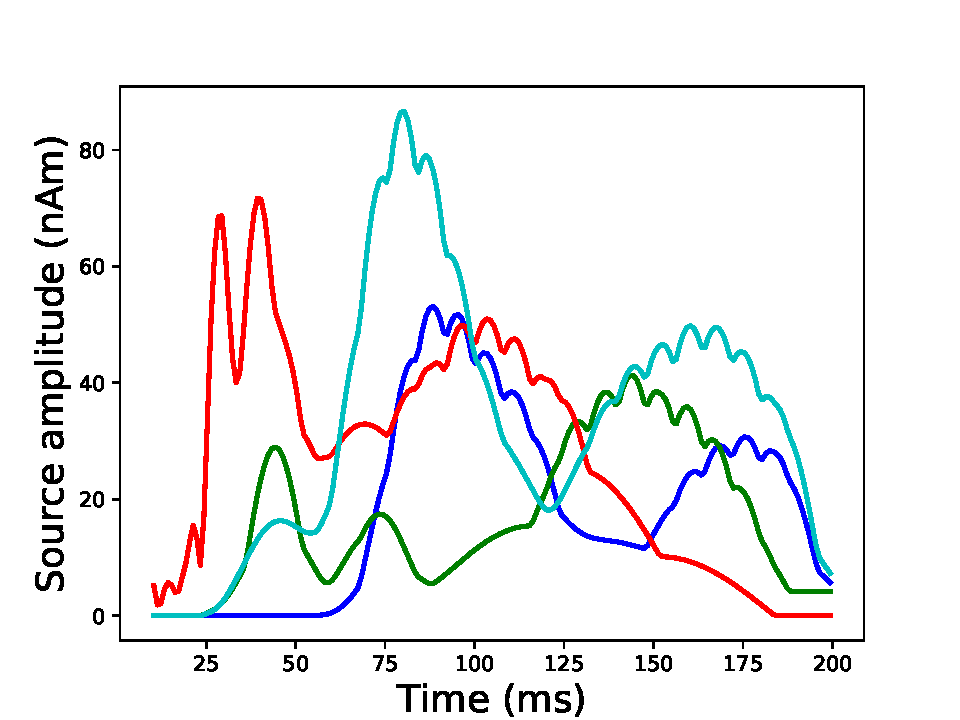
\includegraphics[width=\textwidth]{multidict/stft_ws_64_16_tshift_32_8}
            \caption{STFT: window size = 64-16,\\
            		    time shift = 32-8}
            \label{fig:stft_short}
        \end{subfigure}
        \vskip\baselineskip\vspace{-15pt}
        \begin{subfigure}[b]{0.48\textwidth}   
            \centering 
            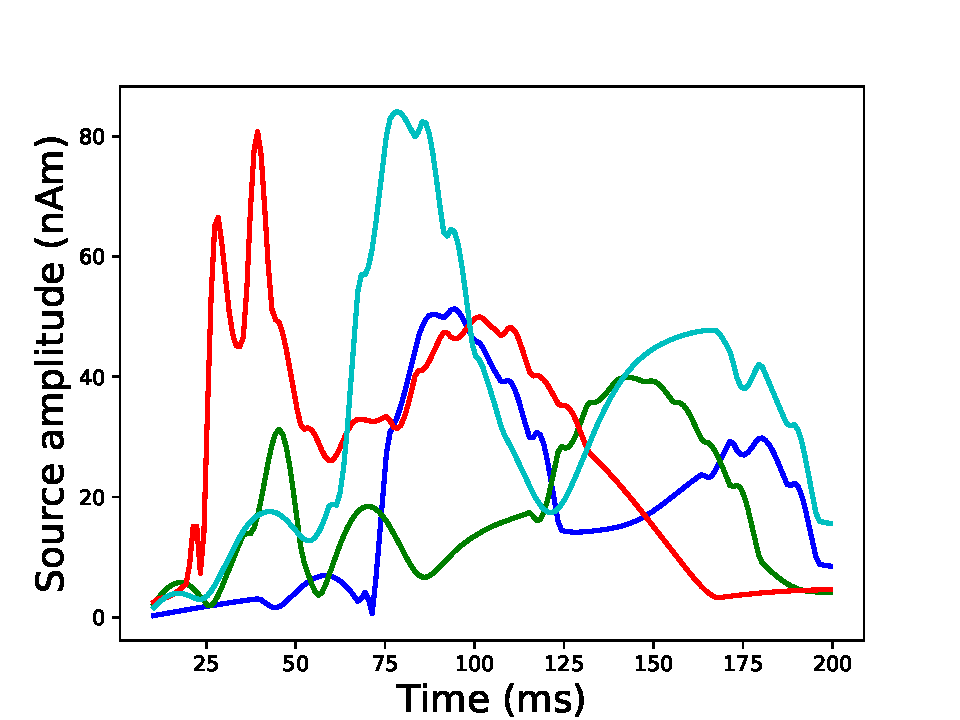
\includegraphics[width=\textwidth]{multidict/mdct_ws_128_16_tshift_64_8}
            \caption{MDCT: window size = 128-16,\\
            		    time shift = 64-8}
            \label{fig:mdct_long}
        \end{subfigure}
        \quad
        \begin{subfigure}[b]{0.48\textwidth}   
            \centering 
            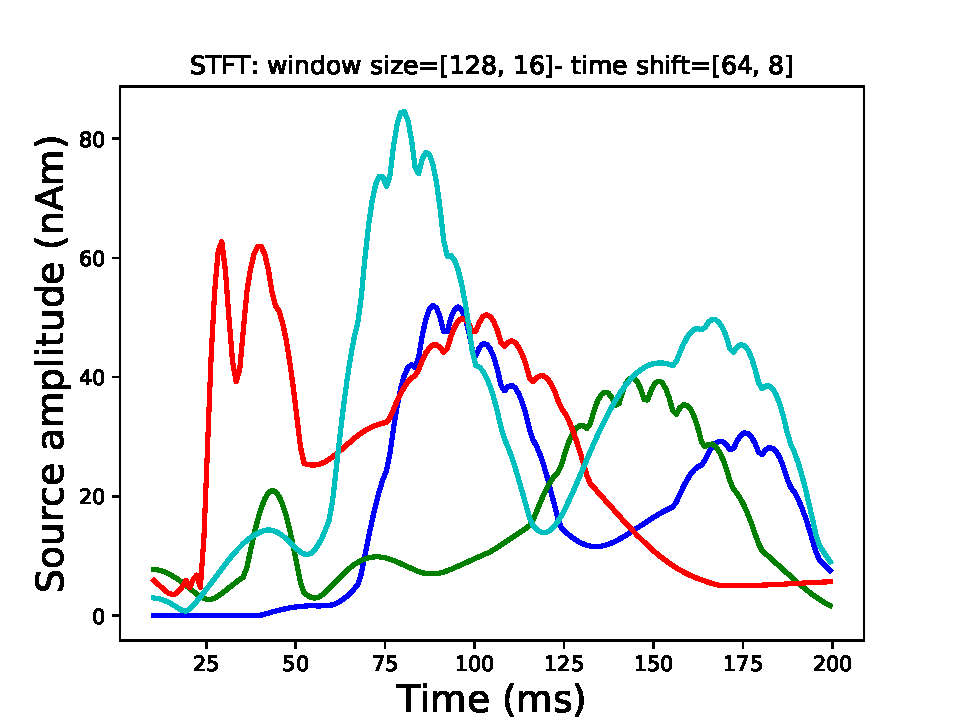
\includegraphics[width=\textwidth]{multidict/stft_ws_128_16_tshift_64_8}
            \caption{STFT: window size = 128-16,\\
            		    time shift = 64-8}
            \label{fig:stft_long}
        \end{subfigure}
        \vskip\baselineskip\vspace{-15pt}
        \begin{subfigure}[b]{0.48\textwidth}   
            \centering 
            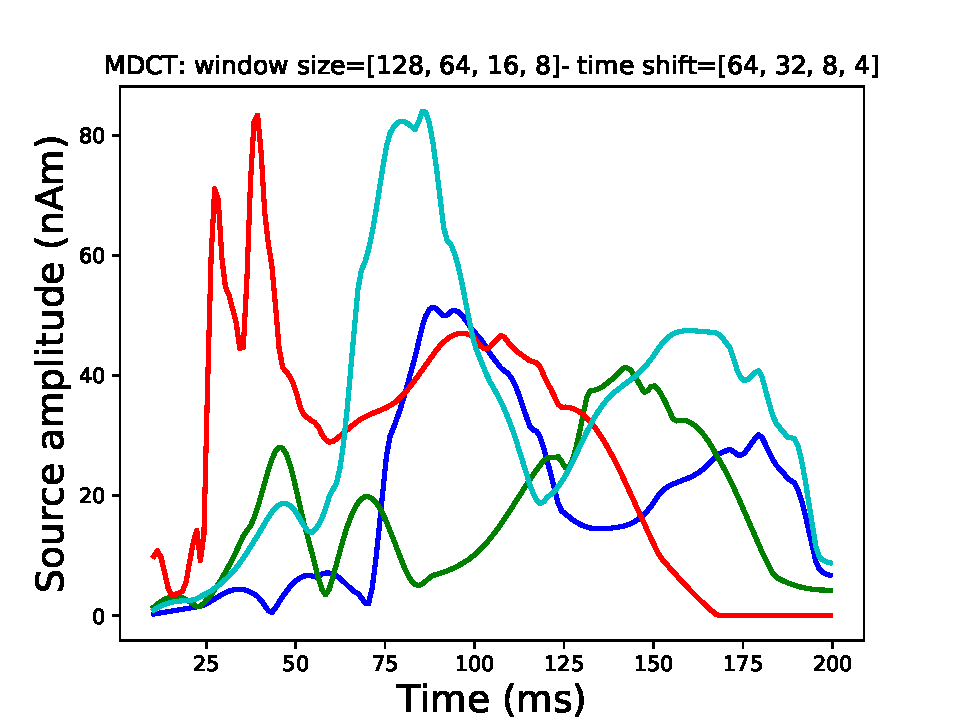
\includegraphics[width=\textwidth]{multidict/mdct_ws_128_64_16_8_tshift_64_32_8_4}
            \caption{MDCT: window size = 128-64-16-8,\\
            		    time shift = 64-32-8-4}
            \label{fig:mdct_all_dict}
        \end{subfigure}
        \quad
        \begin{subfigure}[b]{0.48\textwidth}   
            \centering 
            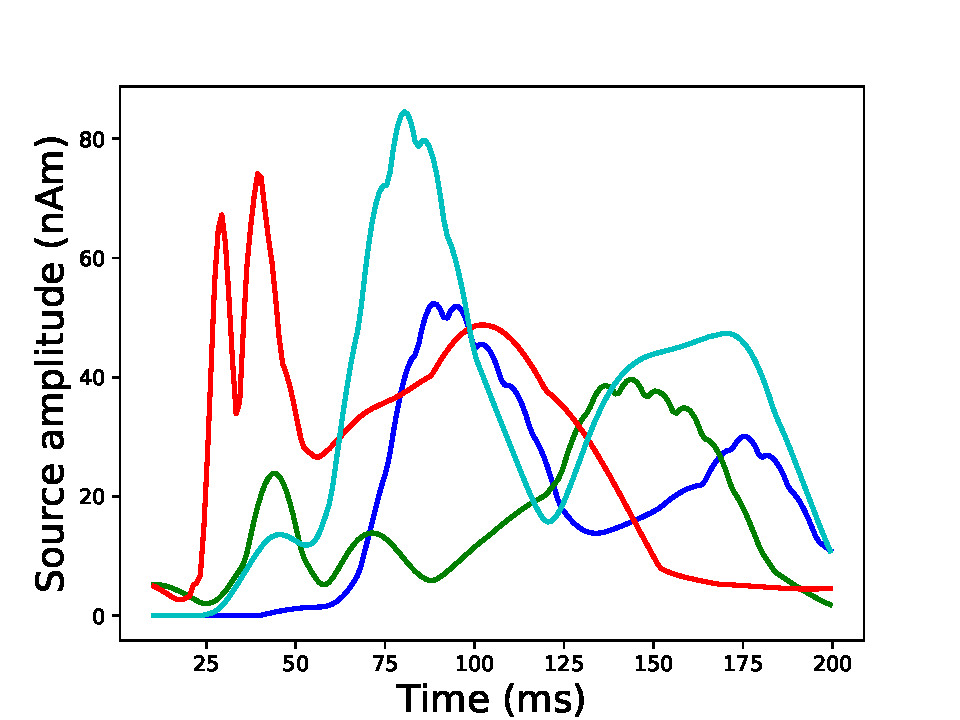
\includegraphics[width=\textwidth]{multidict/stft_ws_128_64_16_8_tshift_64_32_8_4}
            \caption{STFT: window size = 128-64-16-8,\\
            		    time shift = 64-32-8-4}
            \label{fig:stft_all_dict}
        \end{subfigure}
        \caption{Comparison between MDCT and STFT using Somatosensory of the MIND dataset. MDCT is shown in the left column and STFT on the right column.} 
        \label{fig:comparison_mind_mdct_stft}
\end{figure*}

We investigated a second choice: Modified Discrete Cosine Transform (MDCT). The problem found with MDCT is the fact that it is critically sampled. The sliding time windows are overlapping so that the last half of one block coincides with the first half of the next block, \textit{i.e.}, the time shift is equal to the half of the window's length. Figure~\ref{fig:comparison_mind_mdct_stft} shows several mixture of dictionaries for MDCT, but also for STFT if we set the time shift at half the window size. One can directly notice that it is harder to obtain both transient and smooth signals without any leakage between the time sources. MDCT is more sensitive to all the hyperparameters: the dictionary window length and the $\lambda_{space}$/$\lambda_{time}$. Even if we leave in a side the compromise that one needs to keep in mind between the size of multi-scale dictionary and the computation time by having multiple dictionaries concatenated together as in Figure~\ref{fig:comparison_mind_mdct_stft}-\ref{fig:mdct_all_dict}, MDCT is still not able to be comparable to STFT as in Figure~\ref{fig:MEG}.

\section{Conclusion \& Perspective}
In this chapter, the main motivation of the multi-scale dictionary has been presented. The first contribution has been presented which improves the irTF-MxNE solver using a multi-scale dictionary to capture the mixture of the MEG/EEG data. The non-convex optimization problem is solved by iteratively solving the convex weighted TF-MxNE problem using block coordinate descent combined with active set strategy to speed up the convergence.

The benefits of the multi-scale irTF-MxNE have been shown on simulated and MEG somatosensory data. Both experiments confirm that multi-scale irTF-MxNE improves the source estimates, in terms of reduced mixing of the time courses, smoothness and detection of both short transients and slower waves. In contrast, both solvers are efficient regarding active set size and amplitude bias, which is due to the non-convexity of the methods. Hence, the multi-scale irTF-MxNE should be applied to data where a mixture of signals coexist, and when the aim is to acquire focal sources with non-stationary and smooth time courses.

 % (https://www.researchgate.net/publication/301731870_Brain_reading_with_ordered_targets_using_ranking_metric).

Further work related to this chapter can address different points:
\begin{itemize}
%    \item Multi-scale irTF-MxNE investigation in terms of dictionary. So far we have used tight Gabor frames, is it the best choice? Doing some \textit{"exhaustive"} comparison between the STFT used here, Modifed Discrete Cosine Transform (MDCT), and Stockwell transform \textit{a.k.a.} S-Transform will help us better understand the dictionary decomposition of the data.
	\item Multi-scale irTF-MxNE improvement in terms of hyperparameter learning, \textit{i.e.} estimation of the best parameters $\lambda_{space}$ and $\lambda_{time}$. In the standard cases, these parameters are selected by cross-validation or sometimes by using the discrepancy principle. A key contribution in this direction would be to use Bayesian inference techniques to estimate those regularization parameters in a composite norms setting.
    
    \item The source localization in general is computed over an \textit{evoked}, \textit{i.e.} in the MEG/EEG field, the evoked is the mean of several trials of the same experiment. The main purpose is to reduce the noise, \textit{i.e.}, increase the SNR of the signal. At a trial level, \textit{i.e.}, for a lower SNR, how can we improve the source localization? We can constraint the localization with the prior knowledge that all trials are supposed to have the same source estimate.
    
    \item Optimization direction, the idea of incorporating screening techniques presented in a huge amount of papers can help to speed up the convergence, and so the reconstruction time\cite{massias2017safe,massiasgap,fercoq-etal:2015,Ndiaye_Fercoq_Gramfort_Salmon15,ndiaye2016gap,ndiaye2017efficient}.
\end{itemize}

